\subsubsection{Detalles de la actividad}
El correcto instalado de herramientas asegura compatibilidad, productividad, y calidad del software, evitando errores técnicos. Facilita colaboración, pruebas, control de versiones y automatización, creando un entorno homogéneo y estable que agiliza el desarrollo y despliegue del proyecto.
%Enlace del fronted en GitHub \href{https://github.com/brahyanarch/frontend-next-dpsec.git}{https://github.com/brahyanarch/frontend-next-dpsec.git}
Enlace del Backend en GitHub \href{https://github.com/brahyanarch/DpsecGenseg.git}{https://github.com/brahyanarch/DpsecGenseg.git}




\begin{figure}[!htb] 
    \centering 
    \caption{Proyecto en Node.js con Express} 
    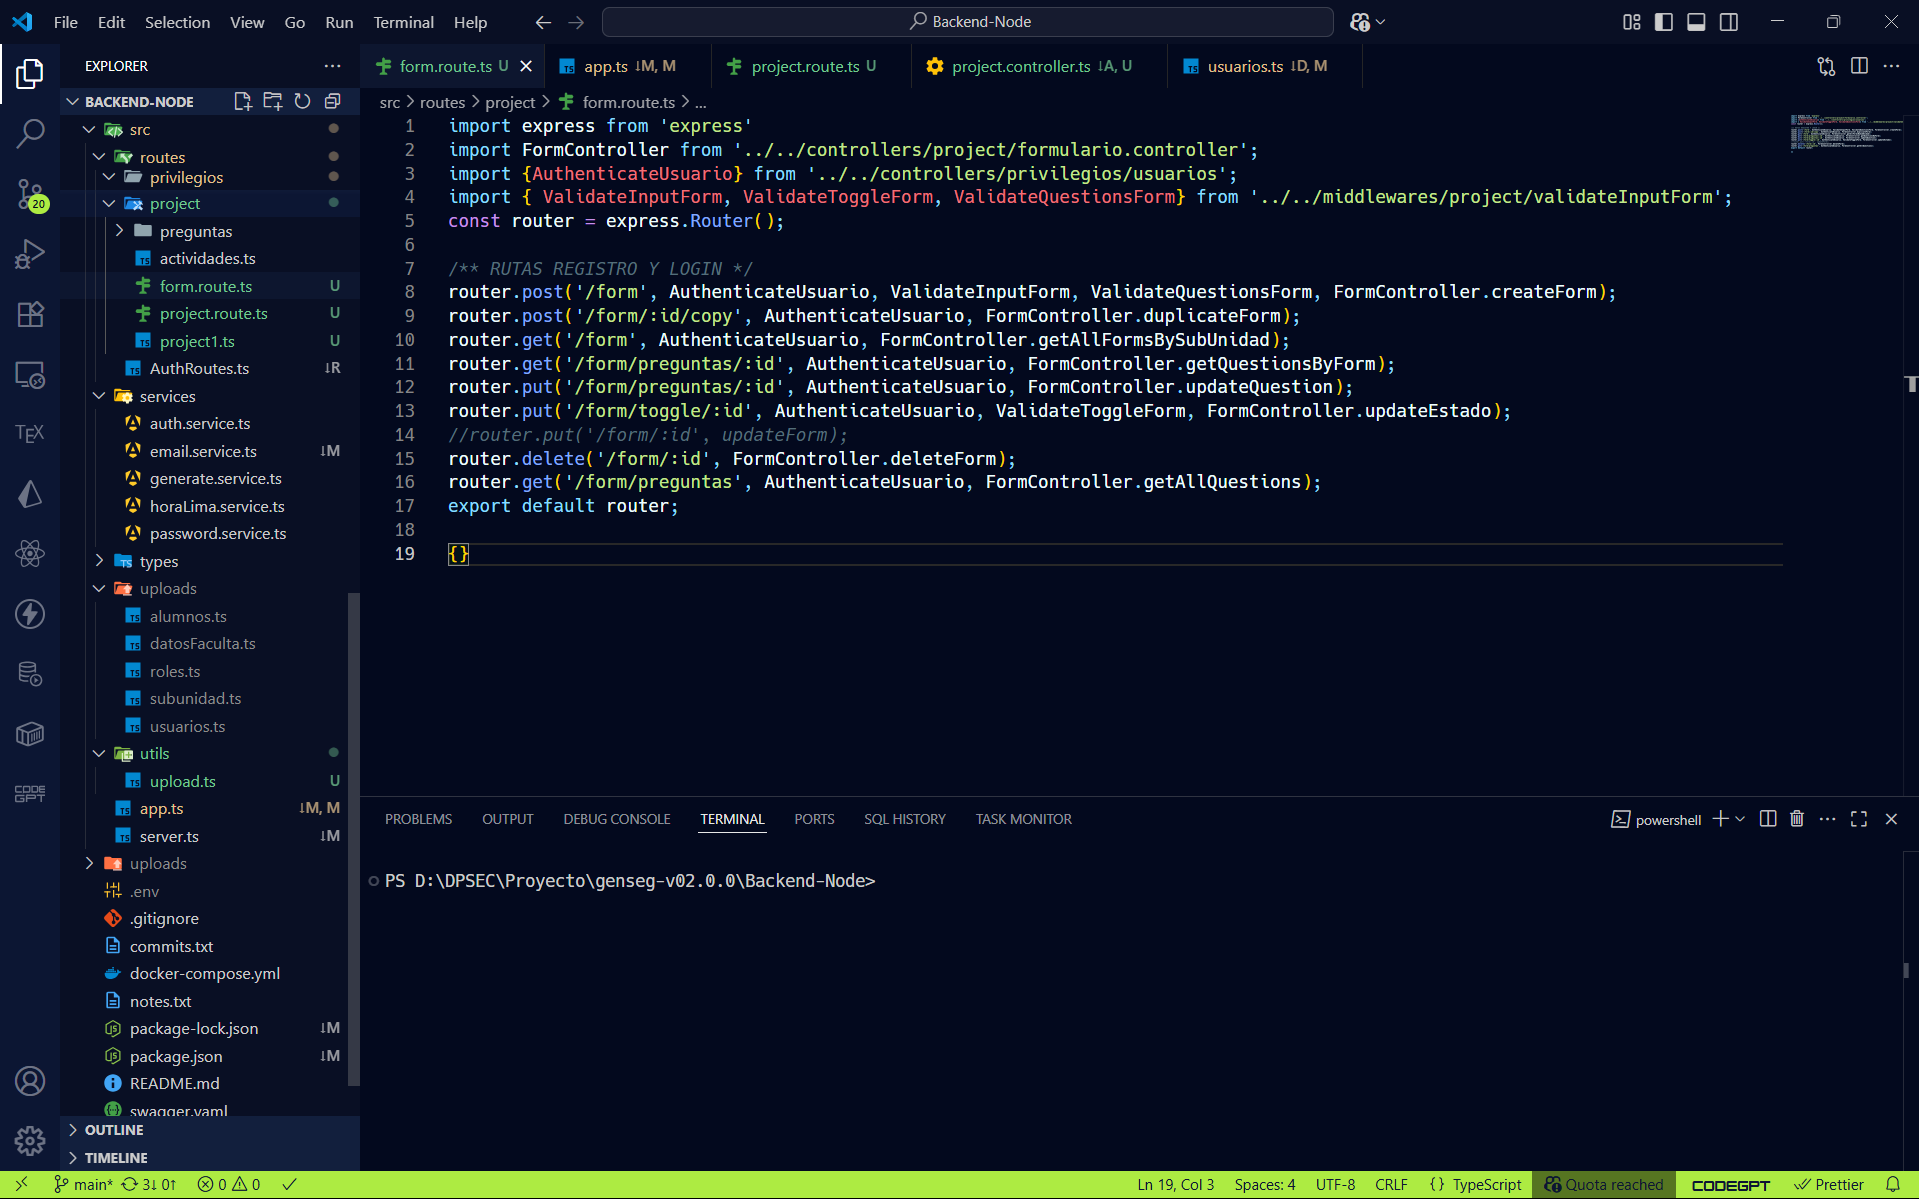
\includegraphics[width=0.9\textwidth]{assets/imagenes/backend.png}
    \label{fig:next} 
\end{figure} 
\FloatBarrier

\begin{figure}[!htb] 
    \centering 
    \caption{Creacion de routes, middlewares y controladores} 
    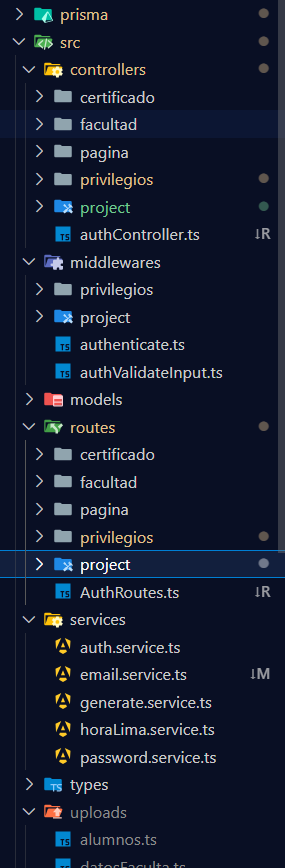
\includegraphics[width=0.2\textwidth]{assets/imagenes/proyecto_backend.png}
    \label{fig:backend} 
\end{figure} 
\FloatBarrier

%\begin{figure}[!htb] 
%    \centering 
%    \caption{Todo okey para trabajar en Next.js} 
%    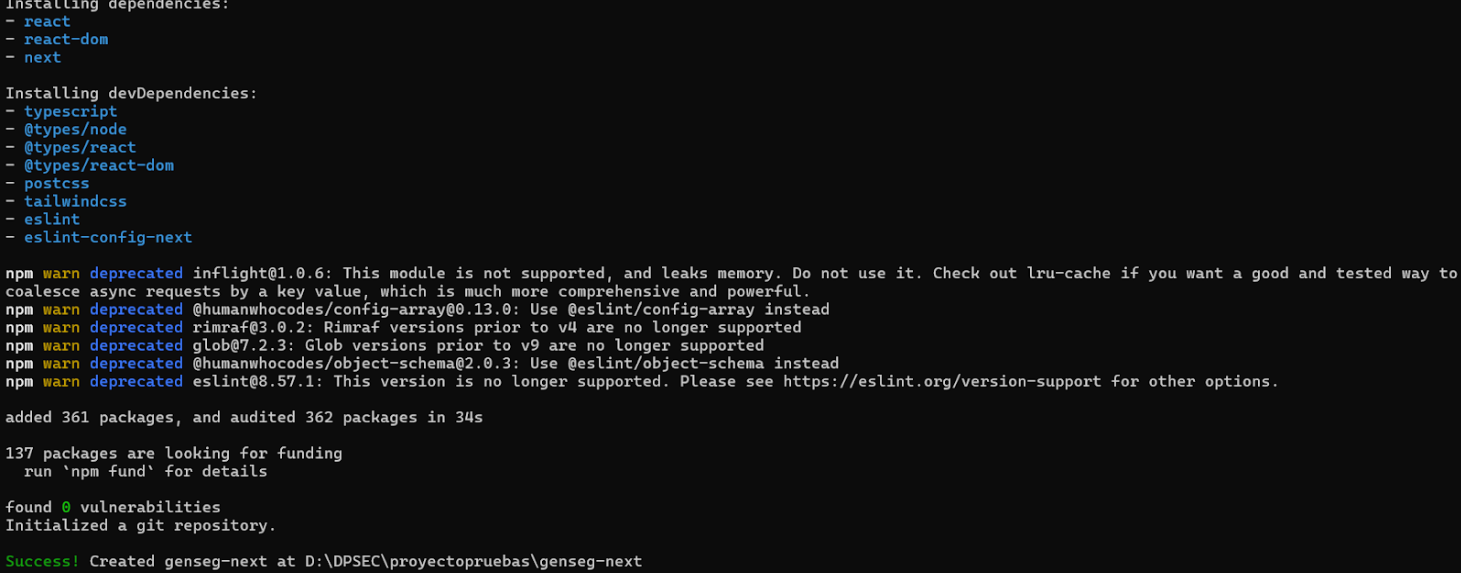
\includegraphics[width=0.8\textwidth]{assets/imagenes/next_listo.png}
%    \label{fig:listo_next} 
%\end{figure} 
%\FloatBarrier


%\begin{lstlisting}[language=Python, caption=Inicializando el proyecto en Next.js, label={lst:next}]
%        > npm run dev
%        
%        > project-genseg@0.1.0 dev
%        > next dev
%        
%         Port 3000 is in use, trying 3001 instead.
%         Next.js 14.2.9
%        - Local:        http://localhost:3001
%        - Environments: .env
%        
%         Starting...
%         Ready in 4.4s
%    \end{lstlisting}


%    \begin{figure}[!htb] 
%        \centering 
%        \caption{Ejecutando en el navegador} 
%        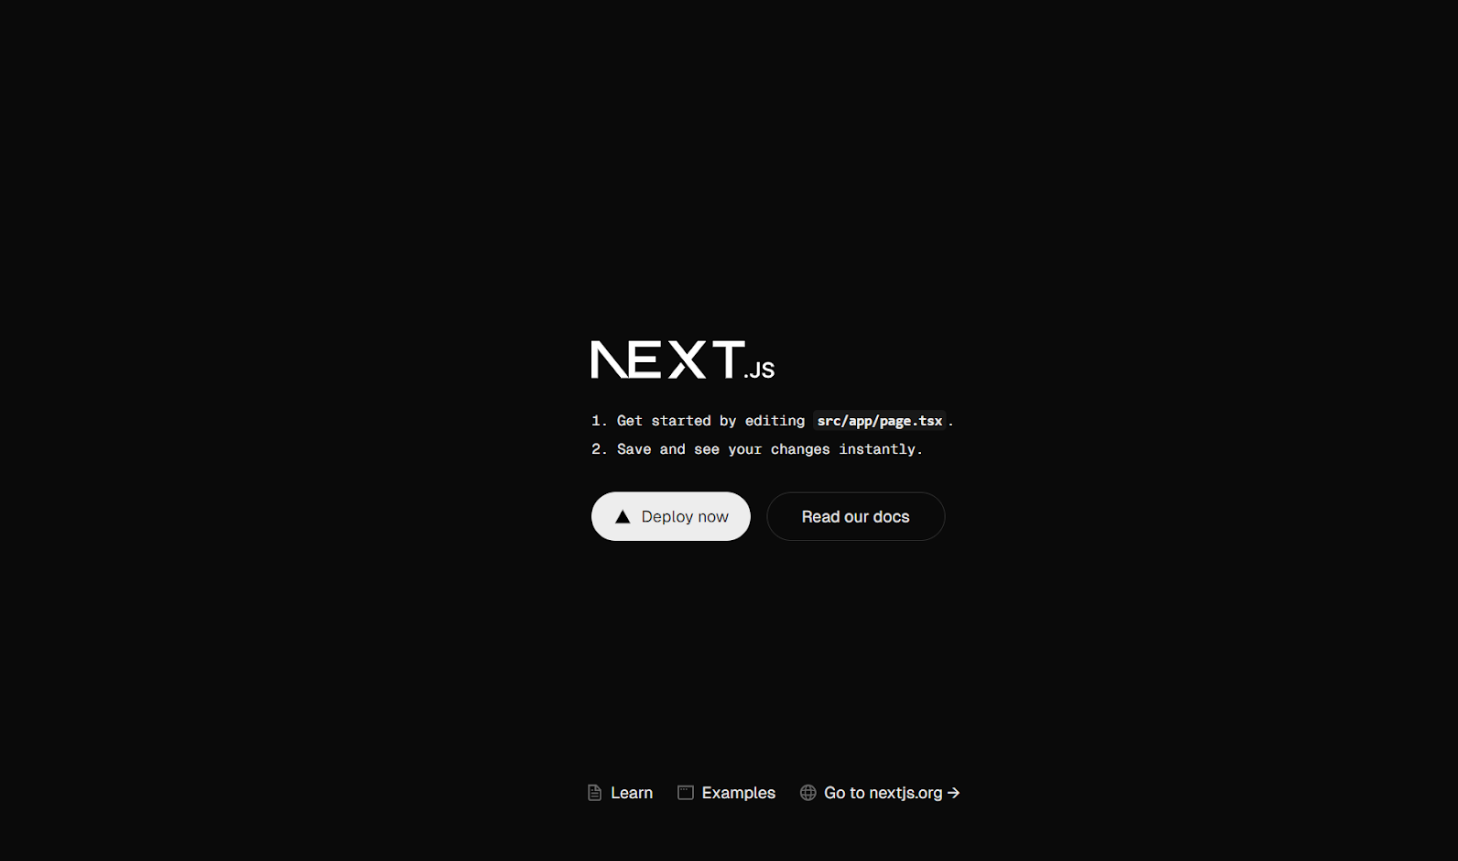
\includegraphics[width=0.8\textwidth]{assets/imagenes/init_next.png}
%        \label{fig:init_next} 
%    \end{figure} 
%    \FloatBarrier
%
%    \begin{figure}[!htb] 
%        \centering 
%        \caption{Codigo en Visual Studio Code} 
%        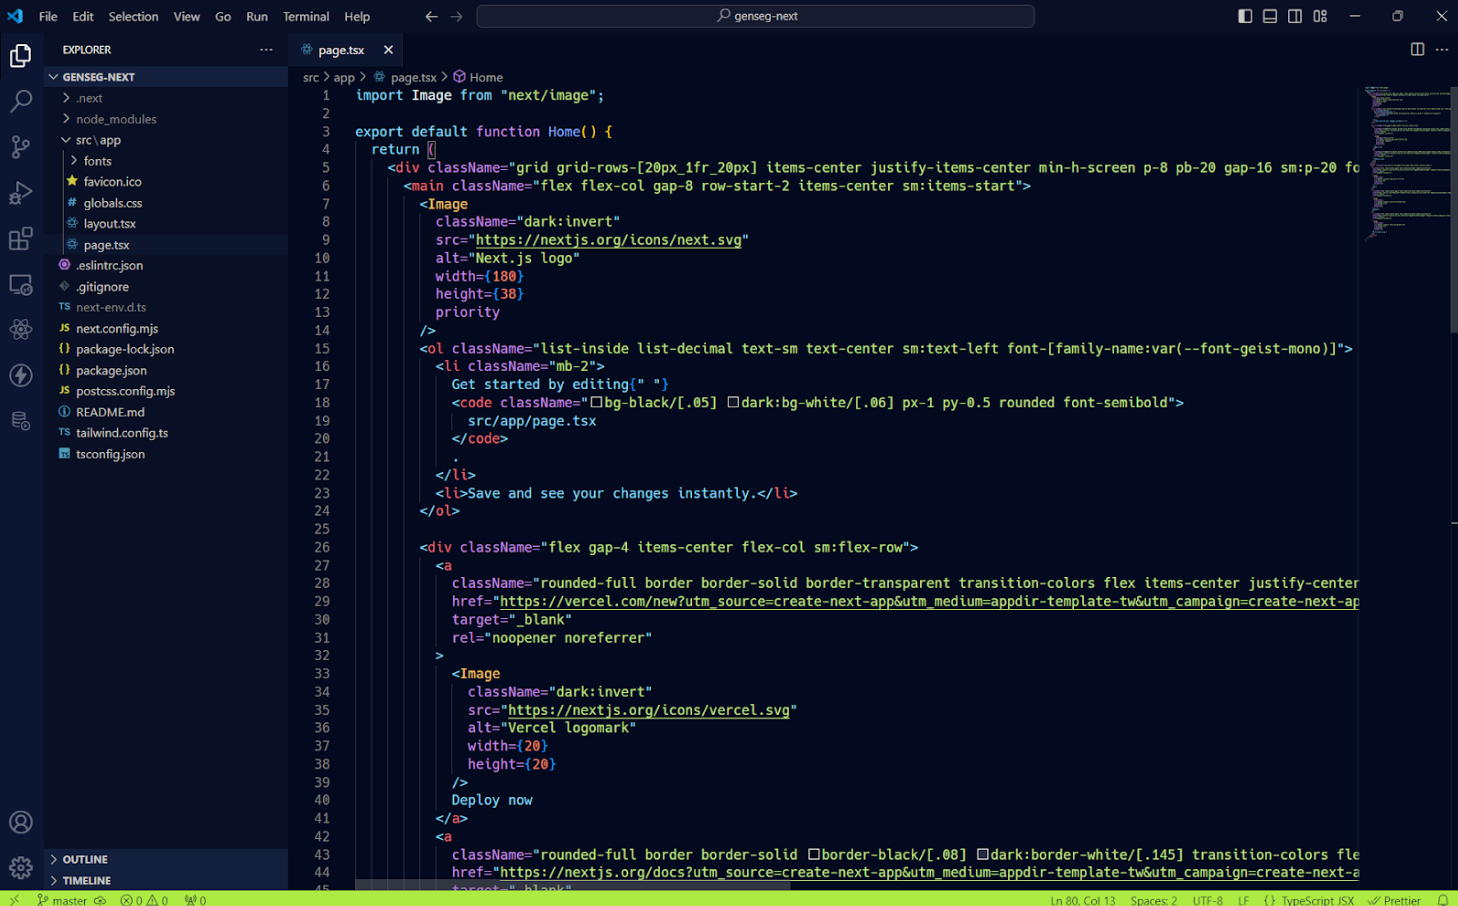
\includegraphics[width=0.8\textwidth]{assets/imagenes/vista_codigo.png}
%        \label{fig:codigo} 
%    \end{figure} 
%    \FloatBarrier
